\documentclass[first=dgreen,second=purple,logo=yellowexc]{aaltoslides}
%\documentclass{aaltoslides} % DEFAULT
%\documentclass[first=purple,second=lgreen,logo=redque,normaltitle,nofoot]{aaltoslides} % SOME OPTION EXAMPLES

\usepackage[latin9]{inputenc}
\usepackage[T1]{fontenc}
\usepackage{graphicx}
\usepackage{amssymb,amsmath}
\usepackage{url}
\usepackage{lastpage}

\newcommand{\bmx}[0]{\begin{bmatrix}}
\newcommand{\emx}[0]{\end{bmatrix}}
\newcommand{\qt}[1]{\left<#1\right>}
\newcommand{\qexp}[1]{\left<#1\right>}
\newcommand{\qlay}[1]{\left[#1\right]}
\newcommand{\vect}[1]{\mathbf{#1}}
\newcommand{\vects}[1]{\boldsymbol{#1}}
\newcommand{\matr}[1]{\mathbf{#1}}
\newcommand{\var}[0]{\operatorname{Var}}
\newcommand{\cov}[0]{\operatorname{Cov}}
\newcommand{\diag}[0]{\operatorname{diag}}
\newcommand{\matrs}[1]{\boldsymbol{#1}}
\newcommand{\va}[0]{\vect{a}}
\newcommand{\vb}[0]{\vect{b}}
\newcommand{\vc}[0]{\vect{c}}
\newcommand{\vh}[0]{\vect{h}}
\newcommand{\vv}[0]{\vect{v}}
\newcommand{\vf}[0]{\vect{f}}
\newcommand{\vx}[0]{\vect{x}}
\newcommand{\vy}[0]{\vect{y}}
\newcommand{\vg}[0]{\vect{g}}
\newcommand{\vr}[0]{\vect{r}}
\newcommand{\vq}[0]{\vect{q}}
\newcommand{\vm}[0]{\vect{m}}
\newcommand{\vs}[0]{\vect{s}}
\newcommand{\vw}[0]{\vect{w}}
\newcommand{\vL}[0]{\vect{L}}
\newcommand{\vp}[0]{\vect{p}}
\newcommand{\mW}[0]{\matr{W}}
\newcommand{\mG}[0]{\matr{G}}
\newcommand{\mX}[0]{\matr{X}}
\newcommand{\mY}[0]{\matr{Y}}
\newcommand{\mK}[0]{\matr{K}}
\newcommand{\mH}[0]{\matr{H}}
\newcommand{\mQ}[0]{\matr{Q}}
\newcommand{\mU}[0]{\matr{U}}
\newcommand{\mR}[0]{\matr{R}}
\newcommand{\mV}[0]{\matr{V}}
\newcommand{\mA}{\matr{A}}
\newcommand{\mD}{\matr{D}}
\newcommand{\mC}{\matr{C}}
\newcommand{\mS}{\matr{S}}
\newcommand{\mI}{\matr{I}}
\newcommand{\mL}{\matr{L}}
\newcommand{\mzero}[0]{\matr{0}}
\newcommand{\td}[0]{\text{d}}
\newcommand{\valpha}[0]{\vects{\alpha}}
\newcommand{\vbeta}[0]{\vects{\beta}}
\newcommand{\vsig}[0]{\vects{\sigma}}
\newcommand{\vmu}[0]{\vects{\mu}}
\newcommand{\vone}[0]{\vects{1}}
\newcommand{\vzero}[0]{\vects{0}}
%\newcommand{\tf}[0]{\text{f}}
\newcommand{\tf}[0]{\text{m}}
\newcommand{\tdf}[0]{\text{dm}}
\newcommand{\TT}[0]{{\vects{\theta}}}
\newcommand{\grad}[0]{\nabla}
\newcommand{\N}[0]{\mathcal{N}}
\newcommand{\CC}[0]{\mathcal{C}}
\newcommand{\QQ}[0]{\mathbb{Q}}
\newcommand{\PP}[0]{\mathbb{P}}
\newcommand{\RR}[0]{\mathbb{R}}
\newcommand{\NN}[0]{\mathcal{N}}
\newcommand{\MM}[0]{\mathcal{M}}
\newcommand{\LL}[0]{\mathcal{L}}
\newcommand{\HH}[0]{\mathcal{H}}
\newcommand{\T}[0]{\mathcal{T}}
\newcommand{\BB}[0]{\mathcal{B}}
\newcommand{\KL}[0]{\text{KL}}
\newcommand{\CD}[0]{\text{CD}}
\newcommand{\sigmoid}{\sigma}
\newcommand{\E}[0]{\mathbb{E}}
\newcommand{\enabla}[0]{\ensuremath{%
    \overset{\raisebox{-0.3ex}[0.5ex][0ex]{%
    \ensuremath{\scriptscriptstyle e}}}{\nabla}}}
\newcommand{\enhnabla}[0]{\nabla_{\hspace{-0.5mm}e}\,}
\newcommand{\tred}[1]{\textcolor{red}{#1}}
\newcommand{\tblue}[1]{\textcolor{blue}{#1}}
\newcommand{\dd}[1]{\text{d}{#1}}

\DeclareMathOperator*{\argmin}{arg\,min}
\DeclareMathOperator*{\argmax}{arg\,max}

\newcommand{\dbm}{DBM}
\newcommand{\dbmptrbm}{DBM$^\text{DBN}_\text{RBM}$}
\newcommand{\dbmptdae}{DBM$^\text{sDAE}_\text{RBM}$}
\newcommand{\dbmptruslan}{DBM$^\text{S\&H}$}
\newcommand{\dbmptruslanrbm}{DBM$^\text{S\&H}_\text{RBM}$}
\newcommand{\dbmptruslanfvbm}{DBM$^\text{S\&H}_\text{FVBM}$}

\title{Learning and Inference in Deep, Unsupervised Neural Networks}

\author[K. Cho]{Kyunghyun Cho}
\institute[ICS]{Department of Information and Computer Science\\
Aalto University, School of Science\\kyunghyun.cho@aalto.fi}

\aaltofootertext{Foundations and Advances in Deep Learning}{\today}{\arabic{page}/\pageref{LastPage}\ }

\date{\today}

\begin{document}

%%%%%%%%%%%%%%%%%%%%%%%%%%%%%%%%%%%%%%%%%%%%%%%%%%%%%%%%%%%%%%%%%%%%%%%%%%%%%%%%%%%%%%%%%%%%%

\aaltotitleframe

%%%%%%%%%%%%%%%%%%%%%%%%%%%%%%%%%%%%%%%%%%%%%%%%%%%%%%%%%%%%%%%%%%%%%%%%%%%%%%%%%%%%%%%%%%%%%

\begin{frame}{Machine Learning is\dots}
    \centering
    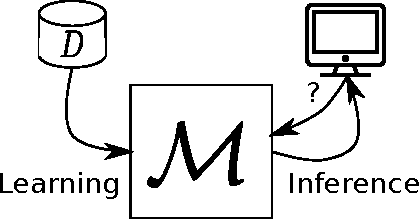
\includegraphics[width=0.55\textwidth]{machinelearning.pdf}

    \vspace{4mm}
    \raggedright
    \begin{enumerate}
        \item Let the model $\MM$ \tred{\textit{learn}} the data $D$
        \item Let the model $\MM$ \tblue{\textit{infer}} unknown
            quantities
    \end{enumerate}
\end{frame}

\begin{frame}{Challenges}
    \centering
    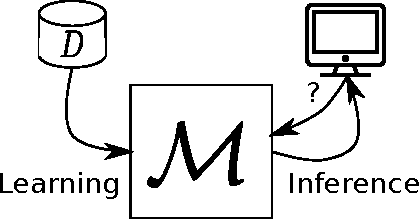
\includegraphics[width=0.55\textwidth]{machinelearning.pdf}

    \vspace{4mm}
    \raggedright
    \begin{enumerate}
        \item \tred{Learning} is \emph{not} trivial 
        \item \tred{Learning} and \tblue{inference} are \emph{not} separate
    \end{enumerate}
\end{frame}

\begin{frame}{Is Learning Optimization?}

    \centering
    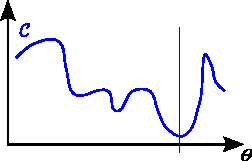
\includegraphics[width=0.5\textwidth]{cost_true.pdf}

    \begin{minipage}{0.48\textwidth}
        \textbf{\emph{Yes}}
    \end{minipage}
    \hfill
    \begin{minipage}{0.48\textwidth}
    %\emph{No}
    \end{minipage}

    %\vspace{1mm}

    \begin{minipage}[t]{0.48\textwidth}
        \vspace{0pt}
    Learning minimizes a cost function $\color{blue}{\CC}$ with respect to
    $\MM$ given a data distribution $p_D$

    \end{minipage}
    \hfill
    \begin{minipage}[t]{0.48\textwidth}
    %    \vspace{0pt}
    %$\color{blue}{\CC}$ is \emph{not} available, but $\color{red}{\tilde{\CC}}$ based
    %on the samples from $p_D$.

    \end{minipage}

\end{frame}

\begin{frame}{Is Learning Optimization?}

    \centering
    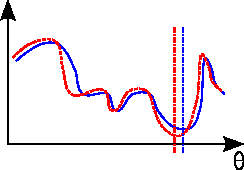
\includegraphics[width=0.5\textwidth]{cost_both.pdf}

    \begin{minipage}{0.48\textwidth}
        \textbf{\emph{Yes}}
    \end{minipage}
    \hfill
    \begin{minipage}{0.48\textwidth}
        \textbf{\emph{No}}
    \end{minipage}

    %\vspace{1mm}

    \begin{minipage}[t]{0.48\textwidth}
        \vspace{0pt}
    Learning minimizes a cost function $\color{blue}{\CC}$ with respect to
    $\MM$ given a data distribution $p_D$

    \end{minipage}
    \hfill
    \begin{minipage}[t]{0.48\textwidth}
        \vspace{0pt}
    $\color{blue}{\CC}$ is \emph{not} available, but $\color{red}{\tilde{\CC}}$ based
    on the samples from $p_D$.

    \end{minipage}

\end{frame}

\begin{frame}{Vicious Cycle or Virtuous Cycle?}

    %\begin{minipage}{0.48\textwidth}
        \centering
        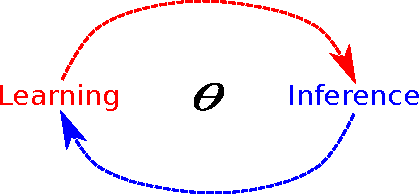
\includegraphics[width=0.5\textwidth]{vicious_cycle.pdf}
    %\end{minipage}
    %\hfill
    %\begin{minipage}{0.48\textwidth}
    %    \tred{\emph{Learning}} which changes $\TT$ requires
    %    \tblue{\emph{inferences}} based on $\TT$. 
    %\end{minipage}

    \vfill
    \raggedright
    Example: MLE for feedforward neural networks
    \begin{align*}
        {\color{red} \min_{\TT} \CC(\TT)} \approx 
        {\color{red} \min_{\TT} \tilde{\CC}(\TT)} =
        {\color{red} \min_{\TT} -\frac{1}{N}\sum_{\left(\vx,t\right) \in D}
        \log {\color{blue}p(y=t \mid \vx, \TT)}}
    \end{align*}

\end{frame}

\begin{frame}{Why is DNN learning considered \emph{more}
    difficult?}
    \begin{itemize}
        \item Learning/Optimization 
            \begin{itemize}
                \item No access to $\CC$, but only to $\tilde{\CC}$
                \item High-dimensional
                \item Non-convex with multiple local minima
                \item Often, intractable to compute (even $\tilde{\CC}$)
            \end{itemize}
        \item Inference
            \begin{itemize}
                \item Often, no analytical expression
                \item Often, intractable to compute
            \end{itemize}
    \end{itemize}
\end{frame}

\begin{frame}{Why is DNN Learning Considered Difficult?}

    \begin{itemize}
        \item Non-convex Optimization with potentially
            \emph{a lot of} local solutions
    \end{itemize}

\end{frame}

\begin{frame}{Avoiding the Learning/Optimization Difficulty}
    \begin{itemize}
        \item Better Optimization Method (General)
        \item Investigating the \emph{structure} of a
            model/problem (Model specific)
    \end{itemize}
\end{frame}


\begin{frame}{}
    \alert{TODO}
\end{frame}

\begin{frame}{Deep Neural Networks: Inspired from Human}

     \centering
     \begin{minipage}{0.37\textwidth}
         \centering
         
\includegraphics[width=0.9\columnwidth]{studying.pdf}

         \small
         \textit{Learn} from massive data
     \end{minipage}

     \vspace{3mm}
     \begin{minipage}{0.37\textwidth}
         \centering
         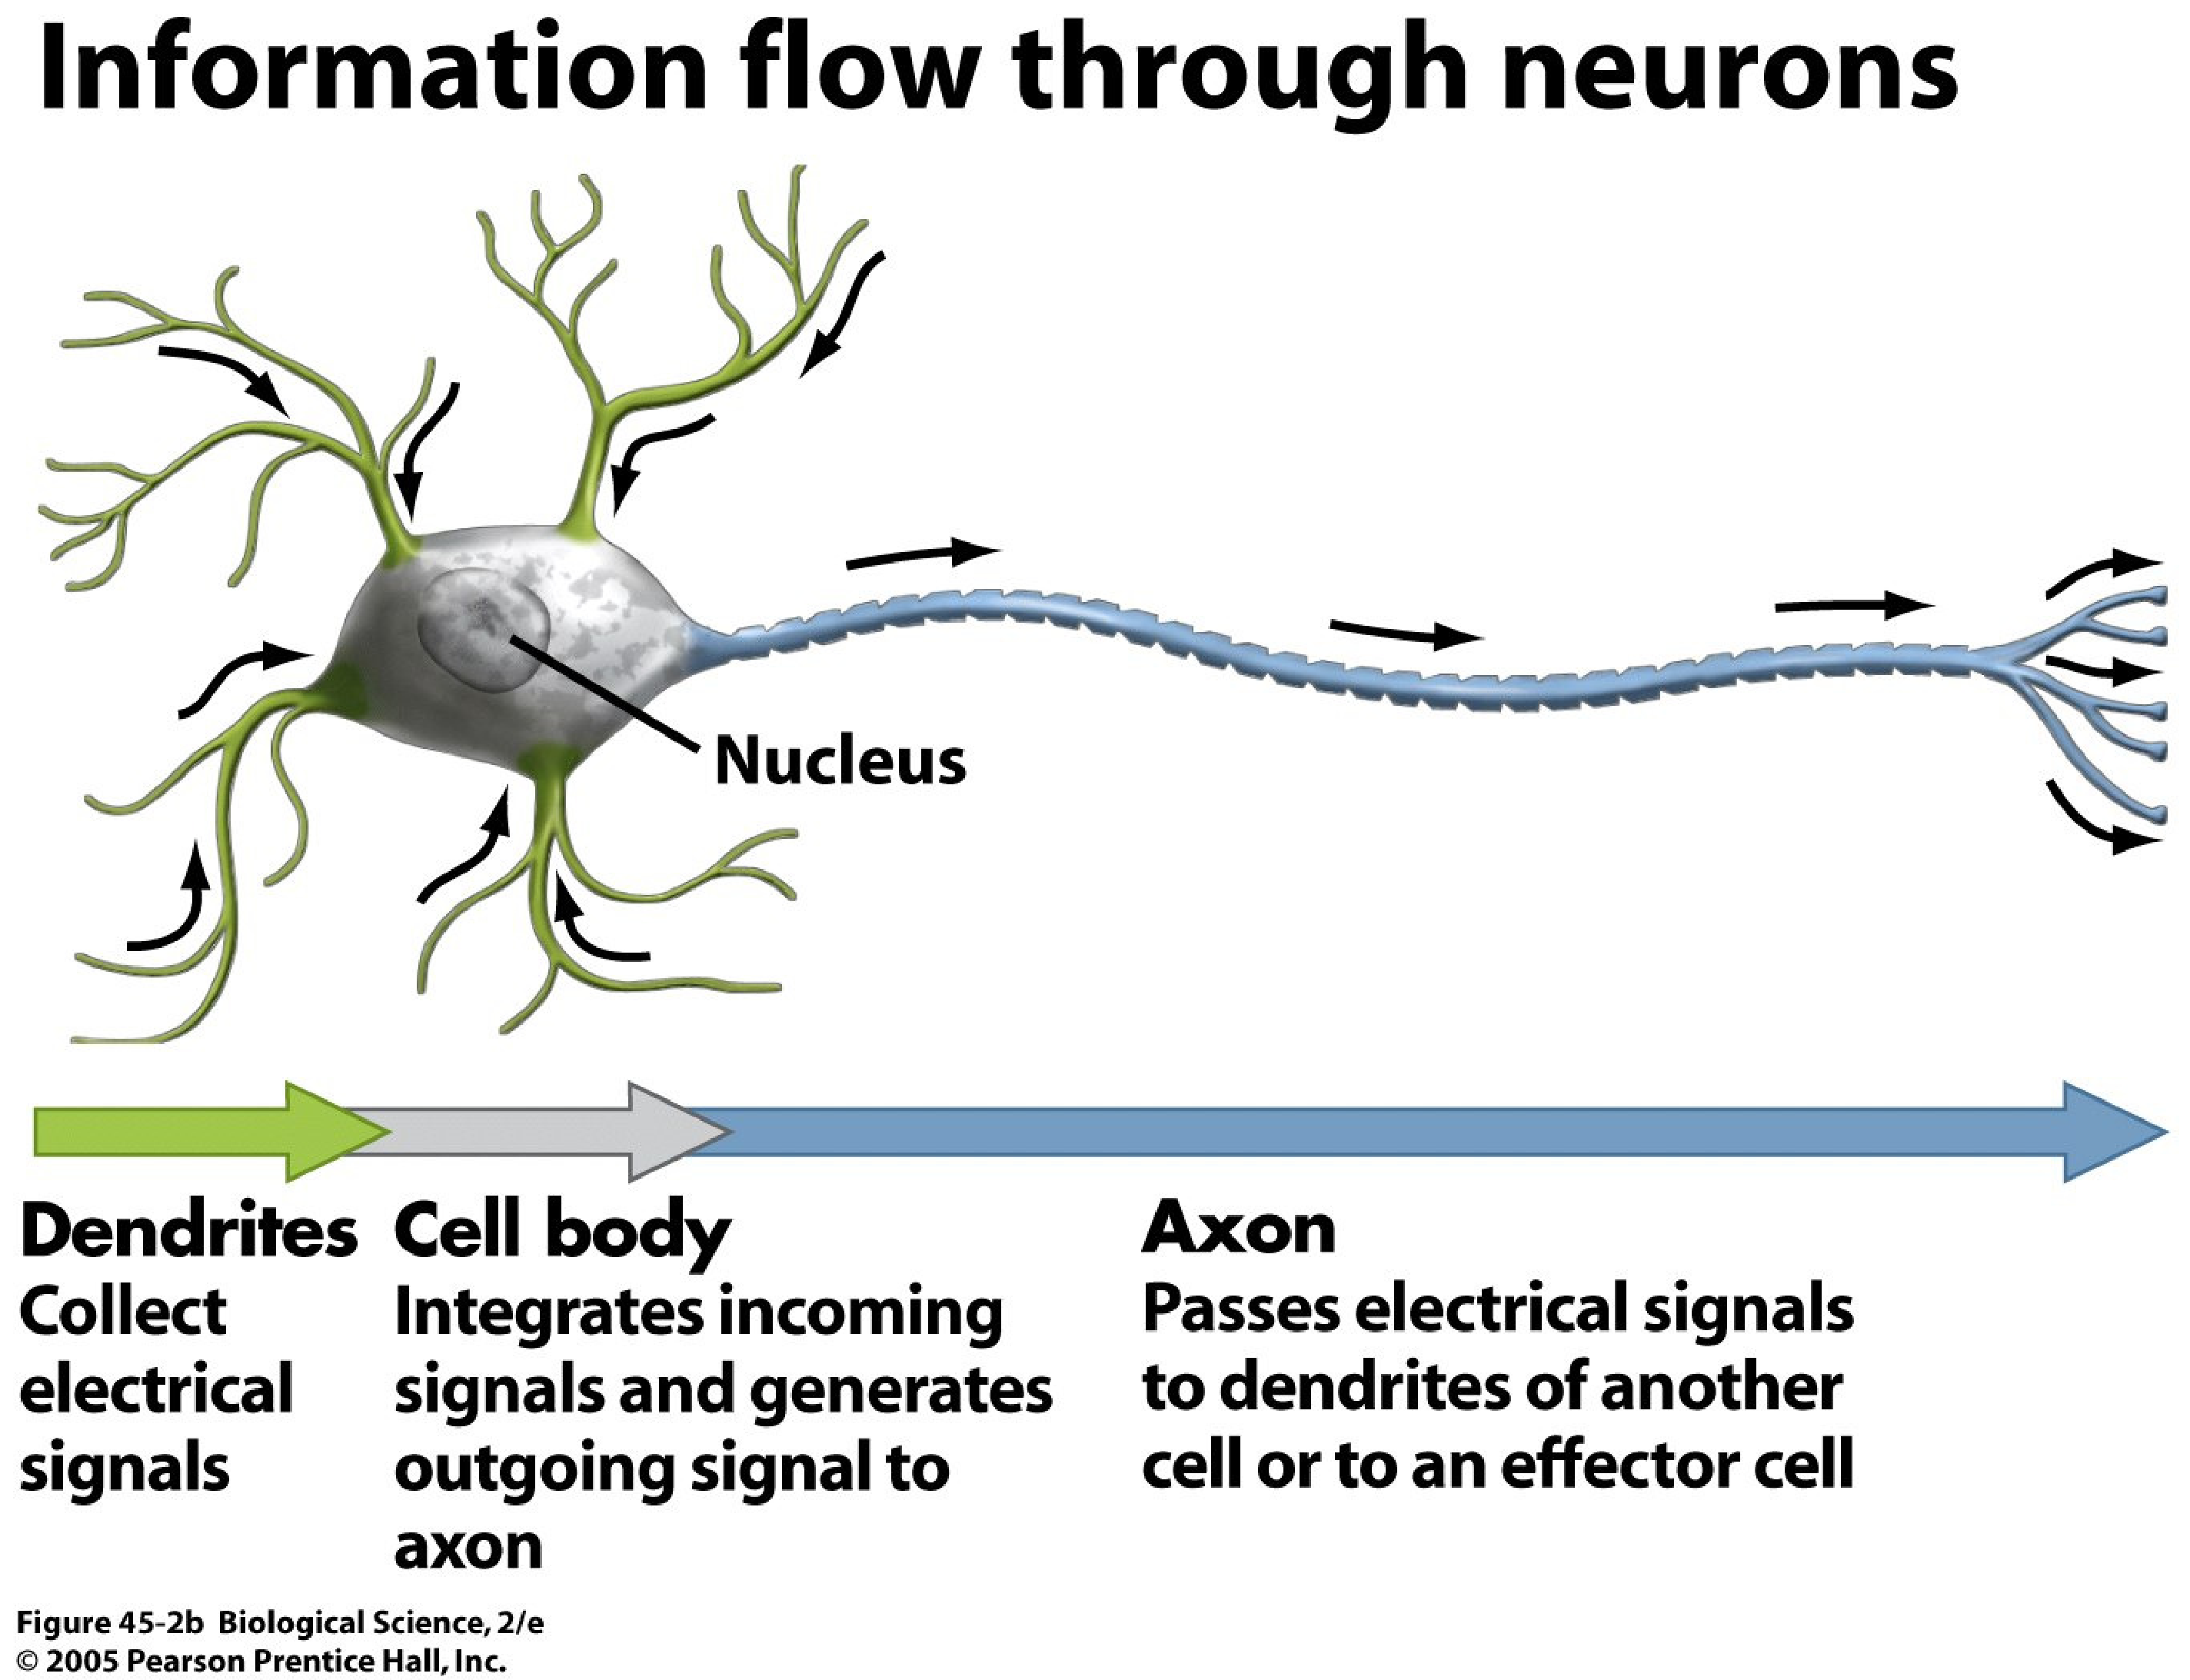
\includegraphics[width=0.9\columnwidth]{neuron.pdf}
     \end{minipage}
     \hfill
     \begin{minipage}{0.37\textwidth}
         \centering
         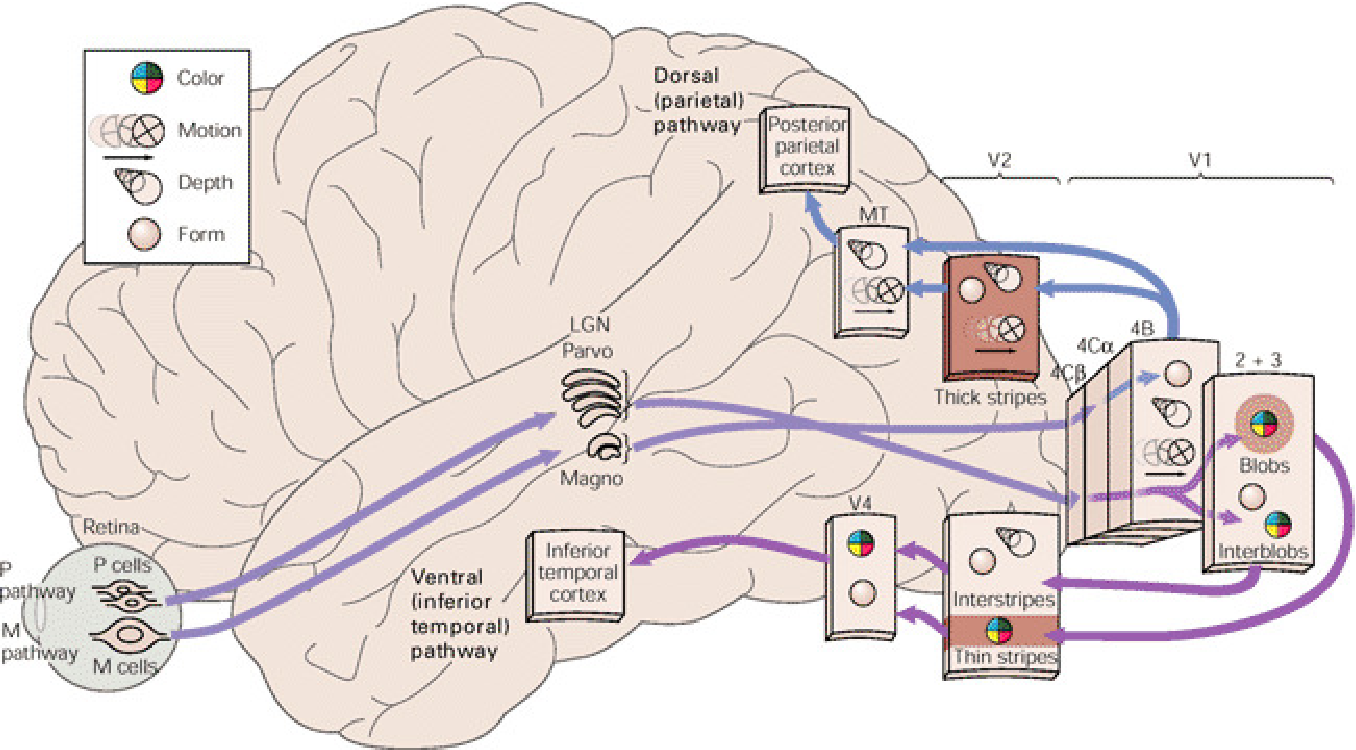
\includegraphics[width=0.9\columnwidth]{visual_pathway.pdf}
         \\
         \raggedleft {\tiny (Van Essen\&Gallant, 1994)}
     \end{minipage}
     \begin{minipage}{0.37\textwidth}
         \centering
         \small
         A network of \textit{simple functions}
     \end{minipage}
     \hfill
     \begin{minipage}{0.4\textwidth}
         \centering
         \small
         \textit{Multi-layered} Processing
     \end{minipage}

\end{frame}


%%%%%%%%%%%%%%%%%%%%%%%%%%%%%%%%%%%%%%%%%%%%%%%%%%%%%%%%%%%%%%%%%%%%%%%%%%%%%%%%%%%%%%%%%%%%%%

%\begin{frame}{Title Page}

%\begin{itemize}
%\item The largest difference to normal Beamer slides is that the title page is produced with a special command \texttt{\textbackslash aaltotitleframe}; this command should be used as it is. \alert{Don't put it in a frame environment!!!} See \texttt{example.tex}.
%\item By default, \texttt{aaltoslides} uses a title page similar to the one in the Aalto Powerpoint templates
%\item A more traditional looking title page can be selected with the option: \texttt{normaltitle}
%\end{itemize}

%\end{frame}

%%%%%%%%%%%%%%%%%%%%%%%%%%%%%%%%%%%%%%%%%%%%%%%%%%%%%%%%%%%%%%%%%%%%%%%%%%%%%%%%%%%%%%%%%%%%%%

%\begin{frame}{Aalto Colors}

%\begin{itemize}

%\item Colors are defined with options: \texttt{first=$\star$} and \texttt{second=$\star$} where $\star$ is one of the following:\\
%{\color{aaltoyellow}yellow}, 
%{\color{aaltored}red}, 
%{\color{aaltoblue}blue}, 
%{\color{aaltogray}gray}, 
%{\color{aaltolgreen}lgreen}, 
%{\color{aaltodgreen}dgreen}, 
%{\color{aaltocyan}cyan}, 
%{\color{aaltopurple}purple}, 
%{\color{aaltomagenta}magenta}, or
%{\color{aaltoorange}orange}

%\item The first color is the primary color (titles, the footer bar, \ldots) and the second color is used in alerted texts and examples

%\item Default colors are: {\color{aaltoblue}blue} and {\color{aaltored}red}

%\item Colors can be used also with the command: \texttt{\textbackslash color\{aalto}$\star$\texttt{\}}. For example, 
%\texttt{\{\textbackslash color\{aaltocyan\}some text\}} 
%gives {\color{aaltocyan}some text}

%\item The rules for choosing colors from the Aalto color circle are not checked (two adjacent colors should not be used)

%\end{itemize}

%\end{frame}

%%%%%%%%%%%%%%%%%%%%%%%%%%%%%%%%%%%%%%%%%%%%%%%%%%%%%%%%%%%%%%%%%%%%%%%%%%%%%%%%%%%%%%%%%%%%%%

%\begin{frame}{Logo}

%\begin{itemize}
%\item \texttt{aaltoslides} supports all variations of the logo:\\[0.2cm]
%
\includegraphics[width=3cm]{Aalto_EN_ScienceandTech_13_RGB_y1.pdf} \hspace{10pt}
%
\includegraphics[width=3cm]{Aalto_EN_ScienceandTech_13_RGB_y2.pdf} \hspace{10pt}
%
\includegraphics[width=3cm]{Aalto_EN_ScienceandTech_13_RGB_y3.pdf} \\[0.2cm]
%
\includegraphics[width=3cm]{Aalto_EN_ScienceandTech_13_RGB_r1.pdf} \hspace{10pt}
%
\includegraphics[width=3cm]{Aalto_EN_ScienceandTech_13_RGB_r2.pdf} \hspace{10pt}
%
\includegraphics[width=3cm]{Aalto_EN_ScienceandTech_13_RGB_r3.pdf} \\[0.2cm]
%
\includegraphics[width=3cm]{Aalto_EN_ScienceandTech_13_RGB_b1.pdf} \hspace{10pt}
%
\includegraphics[width=3cm]{Aalto_EN_ScienceandTech_13_RGB_b2.pdf} \hspace{10pt}
%
\includegraphics[width=3cm]{Aalto_EN_ScienceandTech_13_RGB_b3.pdf} \\
%\item The logo is selected with the option: \texttt{logo=$\star\circ$} where $\star$ is {\color{aaltoyellow}yellow}, {\color{aaltored}red}, or {\color{aaltoblue}blue}, and $\circ$ is either exc, quo, or que for !, ", or ?, respectively; For example, \texttt{logo=yellowquo}
%\item The title page uses a larger variation of the selected logo
%\item By default, the logo is \texttt{logo=redexc}
%\item All logos can be removed with the option: \texttt{nologo}
%\end{itemize}

%\end{frame}

%%%%%%%%%%%%%%%%%%%%%%%%%%%%%%%%%%%%%%%%%%%%%%%%%%%%%%%%%%%%%%%%%%%%%%%%%%%%%%%%%%%%%%%%%%%%%%

%\begin{frame}{Footer}

%\begin{itemize}

%\item By default, the slides have a footer with a logo on the left and an optional three row text\footnote{The first row is highlighted with black by default. To remove this, simply change the color of the first argument of  \texttt{\textbackslash aaltofootertext\{\}\{\}\{\}} with \texttt{\textbackslash color\{aaltogray\}}} on the right
%\item The footer text is set up with the command: \texttt{\textbackslash aaltofootertext\{\}\{\}\{\}}
%\item The footer can be removed with the option: \texttt{nofoot}

%\end{itemize}

%\end{frame}

%%%%%%%%%%%%%%%%%%%%%%%%%%%%%%%%%%%%%%%%%%%%%%%%%%%%%%%%%%%%%%%%%%%%%%%%%%%%%%%%%%%%%%%%%%%%%%

%\begin{frame}{Lengths}

%\begin{itemize}
%\item \texttt{aaltoslides} defines the following lengths: 
%\texttt{\textbackslash aaltofooterplace}, 
%\texttt{\textbackslash aaltofooterruleheight}, 
%\texttt{\textbackslash aaltofooterrulewidth}, 
%\texttt{\textbackslash aaltotitleboxplace},  
%\texttt{\textbackslash aaltotitleboxheight}, 
%\texttt{\textbackslash aaltotitleboxwidth}, 
%\texttt{\textbackslash aaltotitlesep}, 
%\texttt{\textbackslash aaltotitleentrysep}, 
%\texttt{\textbackslash largelogoheight}, and
%\texttt{\textbackslash smalllogoheight} 
%\item The appearance of the slides can be changed by modifying the lengths with \texttt{\textbackslash setlength} or \texttt{\textbackslash addtolength}
%\end{itemize}

%\end{frame}

%%%%%%%%%%%%%%%%%%%%%%%%%%%%%%%%%%%%%%%%%%%%%%%%%%%%%%%%%%%%%%%%%%%%%%%%%%%%%%%%%%%%%%%%%%%%%%


%\begin{frame}{Some Examples}

%\begin{itemize}
%\item Normal text
%\item \alert{Alerted text}
%\end{itemize}

%\begin{block}{Block 1}
%Text
%\end{block}

%\begin{example}
%Text
%\end{example}

%\end{frame}

%%%%%%%%%%%%%%%%%%%%%%%%%%%%%%%%%%%%%%%%%%%%%%%%%%%%%%%%%%%%%%%%%%%%%%%%%%%%%%%%%%%%%%%%%%%%%%

\end{document}
